\newpage
\section{Internet Censorship and Tor}

The following questions concern Tor, and possible attacks against the
anonymity properties that it provides.

\prob{10} 
Recall that each Tor circuit has three relay nodes: a guard, a middle relay,
and an exit node, as shown below. 

\begin{center}
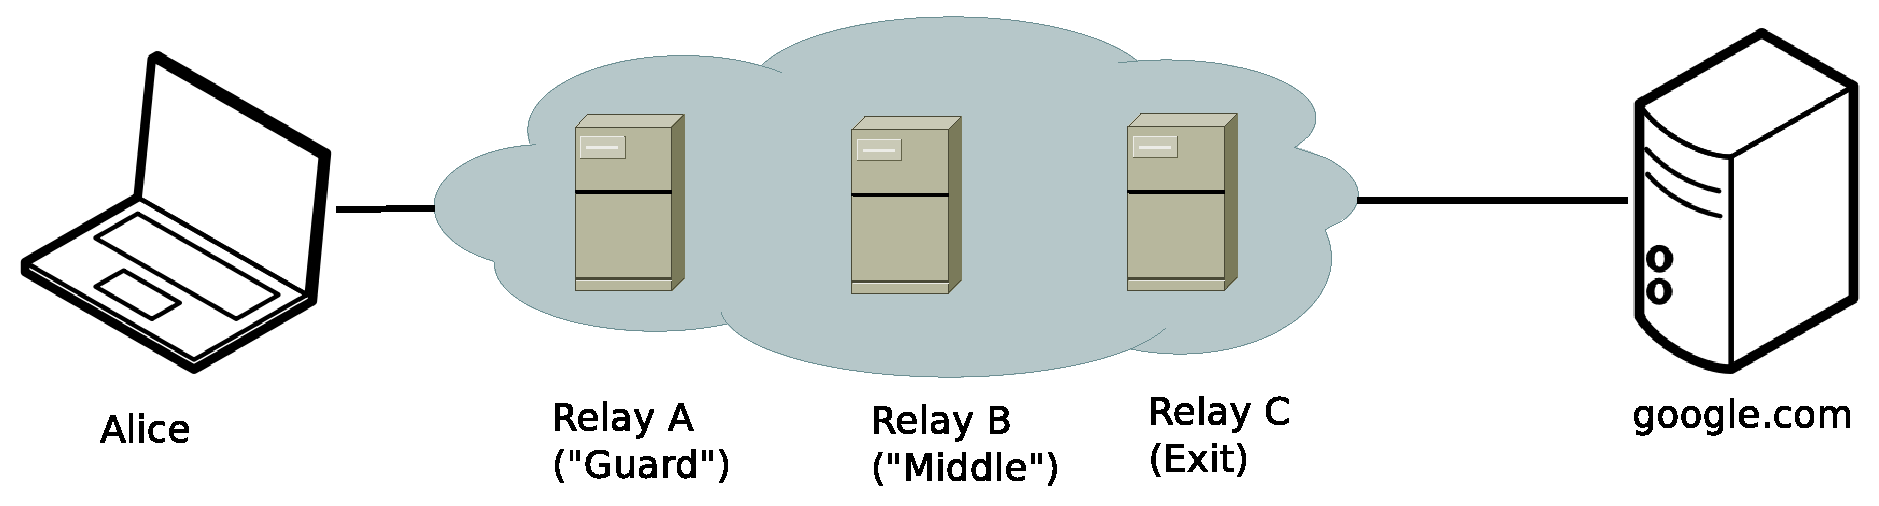
\includegraphics[width=0.65\linewidth]{tor}
\end{center}

Suppose that Alice wants to send a message $m$ to {\tt google.com} through the relays
$A$, $B$, and $C$ below.  {\em Write down the onion encrypted message that Alice's
Tor client would construct.}

Please use the following notation: $\{(A, m)\}_B$ means ``encrypt
$(A,m)$ with $B$'s public key''. $B$ could then decrypt the message $(A,m)$ and
interpret the first part of the tuple as the ``next hop'' $A$, who would receive $m$.  (Hint: Your answer should contain multiple
``onion'' layers of encryption. It should only be one line.)
\eprob

\newpage
\prob{20} 
Recall from lecture that that much of Tor's security depends on
ensuring that no single party has control over multiple nodes, or multiple
parts of the network path between two ends of communication that is taking
place over Tor.  

In class, we talked about Sybil attacks, where an attacker could mount attacks
by controlling multiple {\em relays} in the Tor circuit. This question asks a
related, but slightly different question: What is possible if an attacker can
observe traffic at multiple {\em network observation points} along a path
between two parties communicating over Tor.

Suppose that Alice is a Comcast subscriber and uses Tor to connect to {\tt
google.com} and that her Tor client chooses a circuit with an exit relay that is
{\em also in the Comcast network}.

\begin{enumerate} 
	\item How might Comcast determine be able to determine that Alice is communicating
	with {\tt google.com}? How might it be able to determine the {\em contents}
	of the communication between Alice and {\tt google.com}? 

\item What is a possible defense against the possible attack(s) you
identified in the previous part of the question?
\end{enumerate}

\eprob